\section{Zoo: An NFT Liquidity Protocol}
\label{sec:liquidity-protocol}

Zoo is a liquidity protocol for NFTs, in the way that Uniswap or PancakeSwap is for tokens.

We add new animals to the Zoo ecosystem by deploying new \emph{Drop Contracts}, which define the animal NFT content. Once an Egg NFT hatches, an Animal NFT of the same status is minted and begins to earn \$ZOO tokens according to its staked collateral and the outlined daily reward, determined by its rarity and species.

Based on rarity, age, and how much collateral is added to each NFT, each NFT is effectively an LP token that can be burned to receive the underlying assets (collateral plus rewards earned).

Before freeing the animal --- i.e. burning the NFT --- \$ZOO and practically any currency can be added as liquidity to the animal NFT to increase its value. When users add collateral to their NFT animal, or participate in transactions on the Zoo ecosystem, a small fee is taken to be donated to the Zoo Labs Foundation. Our economics have been designed to cater to the interests of collectors and charities alike, while slowly supporting buy pressure through the gamification of the Zoo game, increasing the value of the total ecosystem.

\paragraph{Pools.} Users can list NFTs as a pool on the marketplace. By placing the NFTs in a pool, the user determines the value of the entire set of NFTs by setting the price of the pool. Once a pool is created, other users can purchase the pool for the value. The buyer must send the amount to the owner to effectively transfer ownership.

\begin{figure}[h]
  \centering
  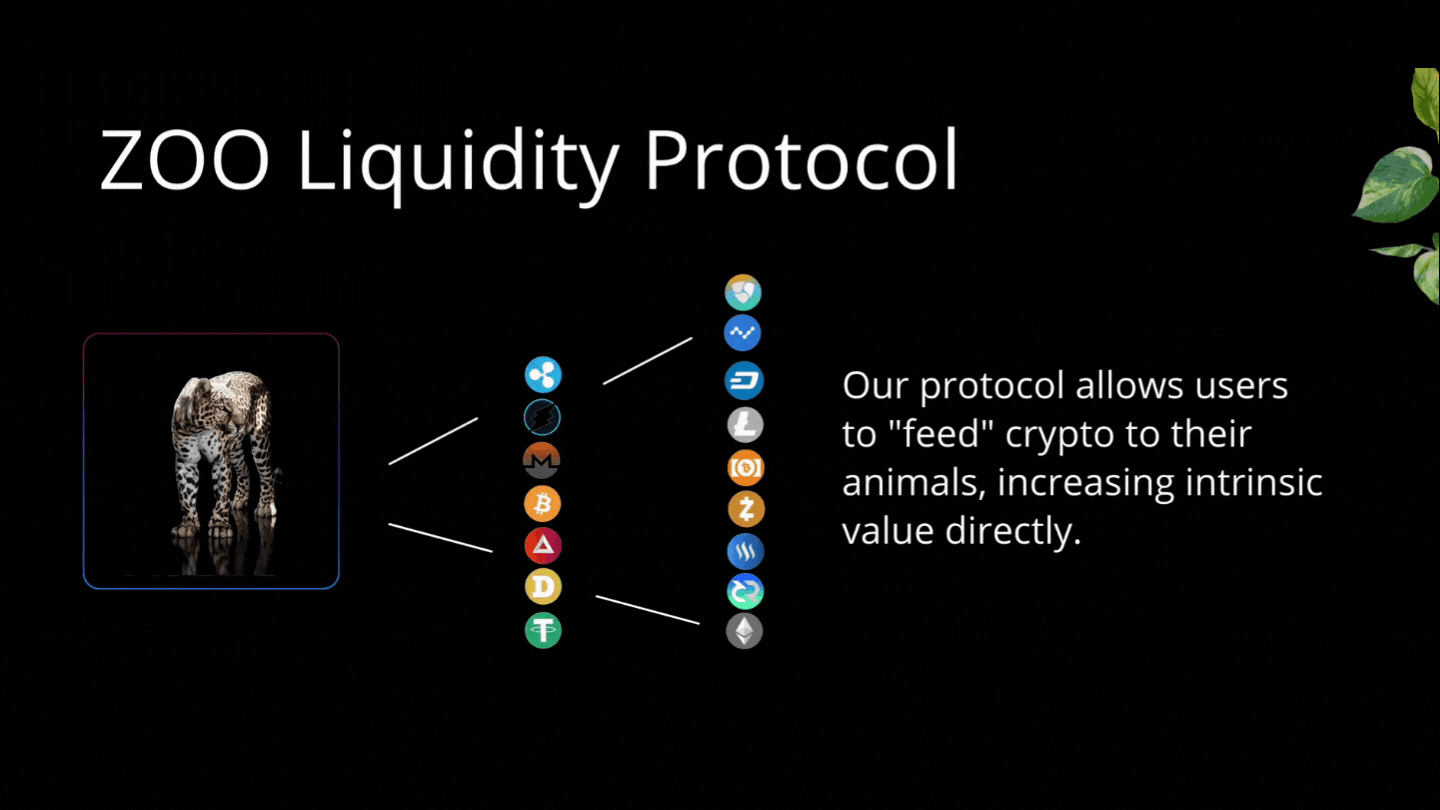
\includegraphics[width=0.85\linewidth]{figures/liquidity-protocol.png}
  \caption{Animated illustration of the NFT liquidity protocol. Egg, baby, teen, and adult forms each represent a position in the protocol; collateral is locked into each NFT and unlockable on burn or transfer.}
  \label{fig:liquidity-protocol}
\end{figure}

\section{NFTs that make you smile}
\label{sec:nfts-smile}

\textit{Transforming digital collectibles into empathetic companions that adapt to users' preferences, emotions, and needs.}

Zoo Labs is forging a revolution in the NFT space, bringing not just awe-inspiring visuals, but also genuine emotional connections into the digital domain. Our goal transcends the standard expectations of NFT collectibles, with the integration of cutting-edge AI, creating intelligent avatars nestled within our virtual animal NFTs.

Enriched with emotional intelligence, our NFTs evolve beyond mere digital assets, emerging as lively companions capable of recognizing and responding to your emotions. They offer engaging dialogues, personalize themselves to your preferences, and deliver companionship reminiscent of an emotional support pet living in your digital ecosystem.

Picture owning an NFT that is not only an enchanting visual representation of a virtual animal but also an empathetic buddy, ready to cheer you up. Our intelligent avatar NFTs are crafted to deliver smiles, brighten your day, and offer emotional solace as you explore the vibrant digital world of Zoo.

Built on advanced AI and intricate language models, our intelligent avatars grow and adapt over time, cultivating distinct personalities and understanding your unique needs. They lend an attentive ear, shower words of encouragement, and offer assistance in daily tasks, truly becoming your digital allies.

By leveraging the power of AI and its APIs, our virtual animal NFTs morph into dynamic companions that understand context and personalize experiences. This unique blend of AI and virtual creatures separates us from conventional NFTs, facilitating a personalized and interactive experience that expands beyond the norms of traditional gaming. With continuous AI advancements and state-of-the-art language model integrations, we continually enhance the intelligence and abilities of our avatar animals.

Combining AI, NFTs, and gaming, we are redefining digital entertainment and promoting profound emotional connections within the virtual realm of Zoo.

\section{Bridging Blockchains}
\label{sec:bridge}

As the DeFi space continues to experience exponential growth, the number of blockchains available for investment also increases. However, each blockchain has its characteristics, with some being easy to use but expensive in fees, while others have light fees but are complex to navigate. The transaction limitations and difficulties experienced through Binance Smart Chain --- on which our token was initially launched --- can be alleviated by our team's efforts in developing a bridge between Binance, Ethereum, and virtually every other blockchain with mass adoption, facilitated by \$ZOO. This bridge, established through our Zoo platform, will facilitate universal exchange within the blockchain space.

While traditional bridges trap tokens in vault contracts, the Zoo Bridge Protocol implements a different approach, leveraging a threshold signature scheme. Oracles monitor the blockchain network to ensure funds are deposited in the smart contract, with \$ZOO tokens being burned on one chain via our bridge protocol and minted on the desired chain. This eliminates the need for a vault contract that could potentially contain vulnerabilities exploitable by attackers. The Zoo Bridge is entirely secured by cross-chain multi-party computation (MPC) validators who operate with threshold signature schemes (TSS).

The network is leaderless and ensures security through each validator running the same process upon receiving on-chain events on the various chains that the MPC validator group tracks. Consensus is achieved when two-thirds of all validators collectively sign the same transaction using their key share, and a trade is issued to the destination chain. The \$ZOO is minted when enough oracles see the underlying asset deposited into the smart contract. In a standard transaction --- such as when \$ZOO teleports from Binance to Ethereum --- we wait for three network confirmations.

\begin{figure}[h]
  \centering
  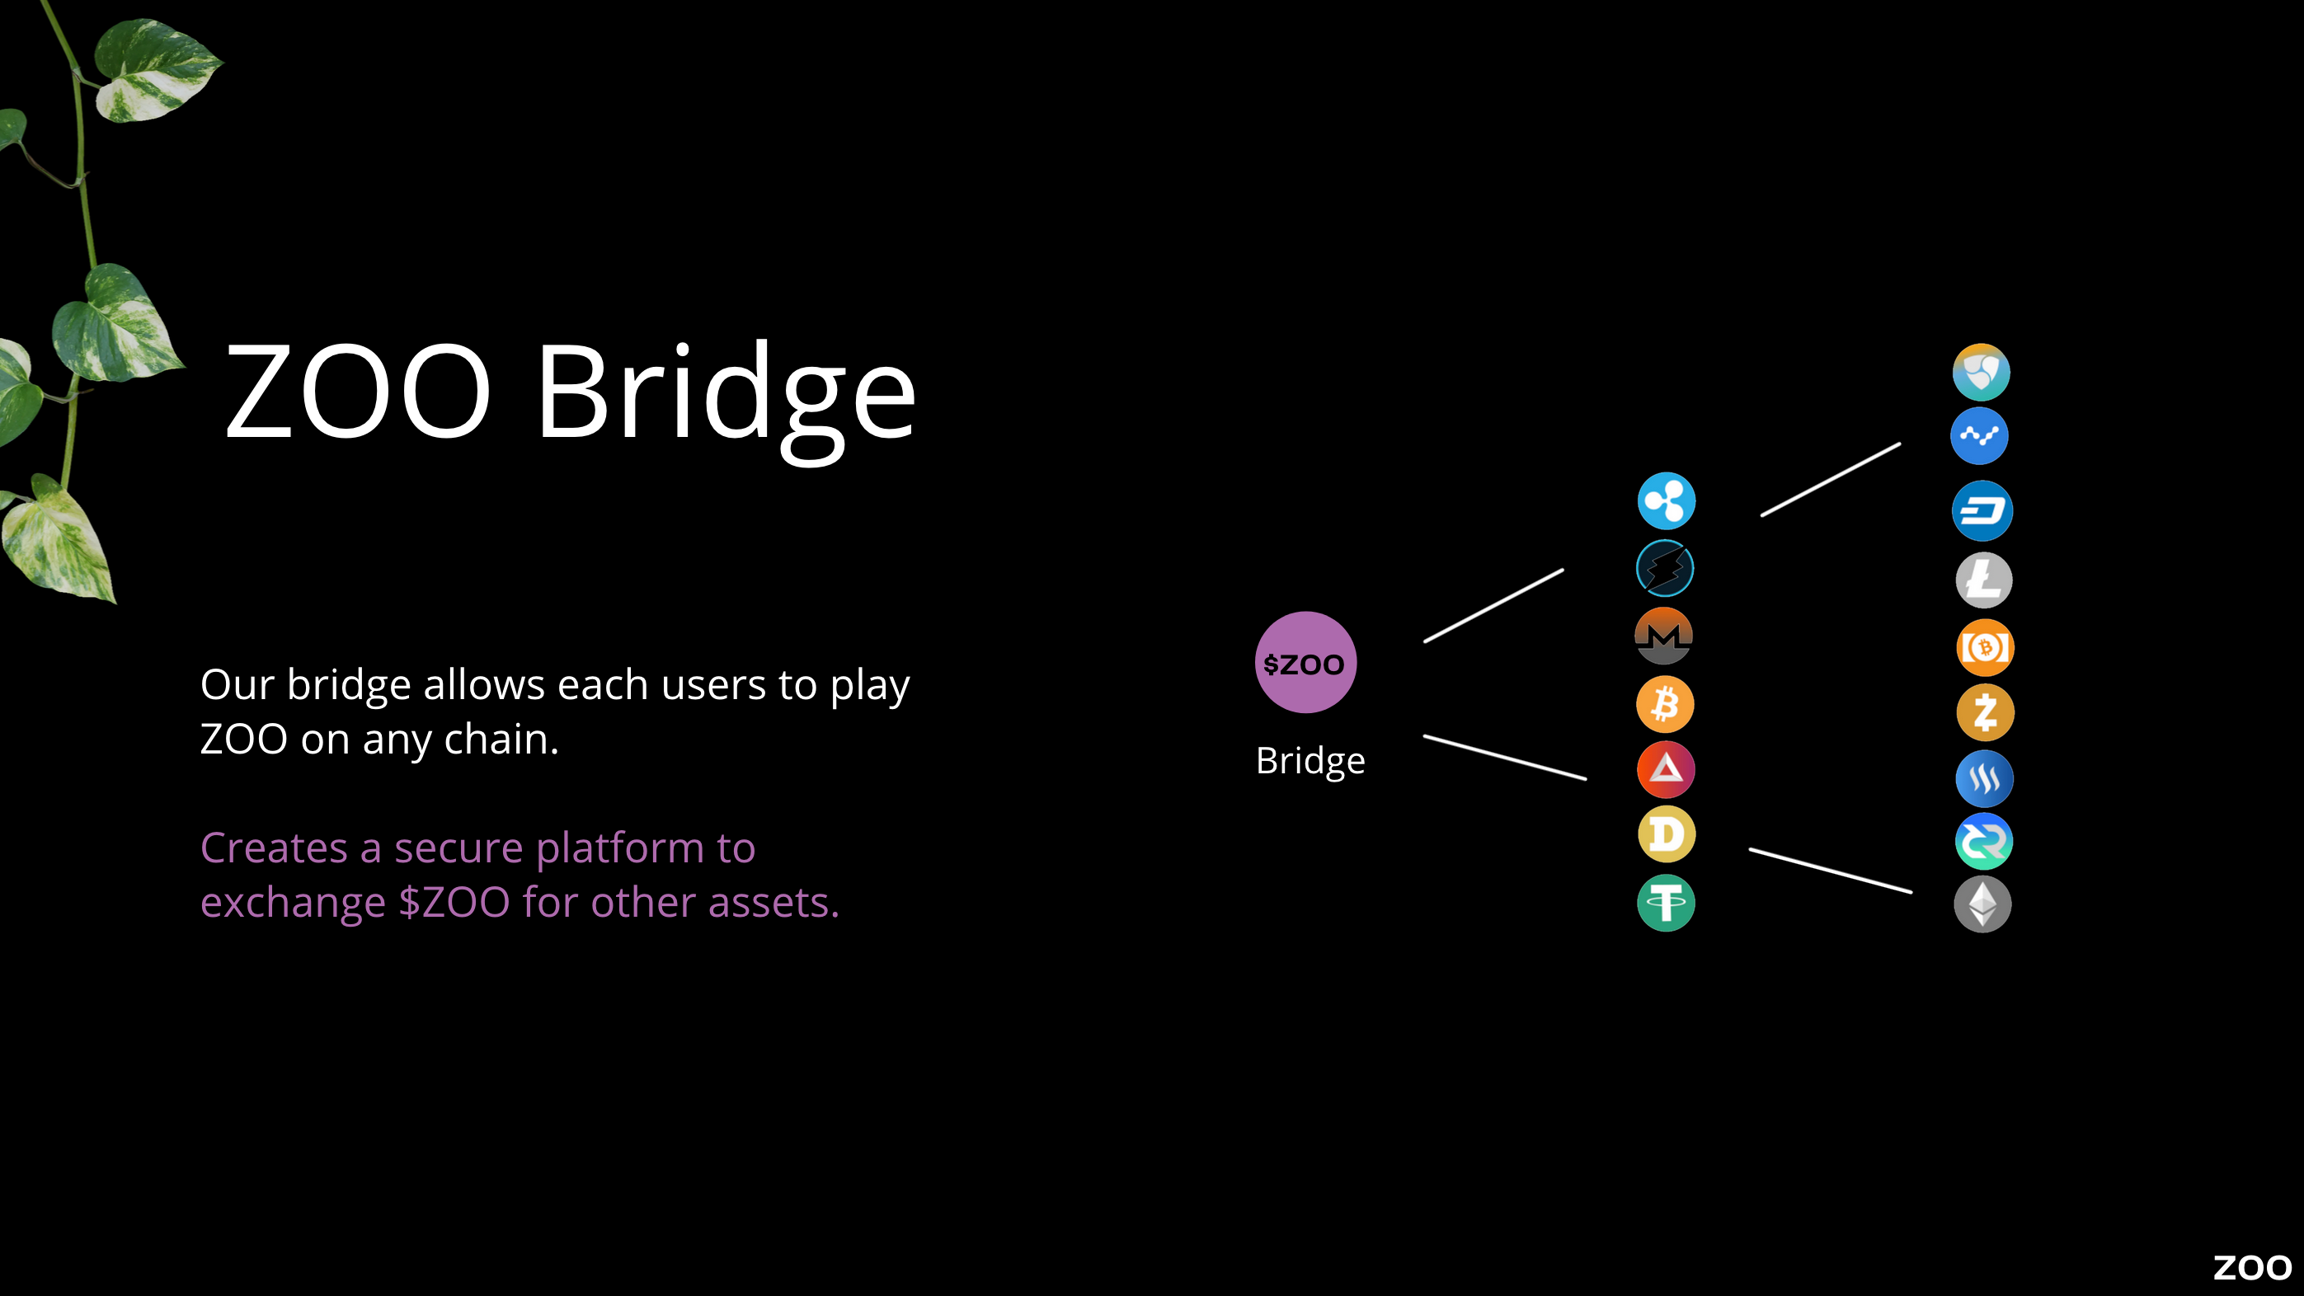
\includegraphics[width=0.9\linewidth]{figures/bridge.png}
  \caption{Zoo Bridge Protocol architecture: MPC validators with threshold signatures replace single-vault custody. Burn-and-mint via two-thirds quorum.}
  \label{fig:bridge}
\end{figure}

\section{Zoo DAO}
\label{sec:dao}

By joining the Zoo DAO, members earn experience points (XP) and governance tokens (KEEPER) to participate in the protocol.

At the heart of the Zoo Protocol lies the Zoo DAO, a community-driven initiative dedicated to preserving endangered species from the brink of extinction. Not only does this movement offer rewarding experiences, but it also empowers members to shape the future of the Zoo Protocol through meaningful decisions.

Zoo DAO governs the Zoo Protocol --- a sophisticated set of smart contracts for collateral-backed NFT animal assets. When you join the Zoo DAO, you earn XP and KEEPER tokens, empowering you to participate actively in the protocol.

The accrual of XP tokens is tied to undertaking \emph{quests} or tasks, each with a specific reward allocation of XP and KEEPER tokens. These quests vary in complexity, with higher-level tasks requiring more substantial contributions to the community and yielding more XP. The more XP earned, the faster a member advances through the ranks. Level is determined by the equation: \texttt{level = (XP + 500) / 300}.

Progressing through the levels not only grants greater authority within the ecosystem, but it also broadens influence. XP tokens are non-transferable and strictly tied to our Decentralized Identification Services (DIS) and comprehensive KYC procedures, preserving the integrity of the system.

Votes are open for all members; however, some voting privileges are reserved for members of certain levels. Higher-level votes are more privileged and controlling. Specific actions --- proposing, voting, and interacting with governance mechanisms --- may call for a blend of \$ZOO and KEEPER tokens. Different proposals cater to different levels, underlining the ecosystem's commitment to inclusivity.

Central to the Zoo Governance and Voting Protocol is the vZOO level and the stake-age duration. Unique to our system, KEEPER token holders \emph{bet} on proposals rather than voting. Winning bets yield additional tokens, promoting active participation. Anyone meeting the requirements may submit a proposal; those gaining traction advance to the next round, while lesser-supported ones are eliminated. This distinctive approach rewards active participation and fosters continuous community involvement.
